\section{Conception}
\subsection{Le chassis}
Le chassis est en profile aluminum. Plusieurs solutions se sont %
présentées :\begin{itemize}%
\item{utiliser du profile pour la construction modulaire}%
\item{utiliser du profile carré}%
\item{utiliser les profiles que propose une célèbre enseigne française %
blanche et verte (fig. \ref{profile} page~\pageref{profile})}
\end{itemize}%
\begin{figure}
   \caption{\label{profile} profile aluminium 23.5 x 23.5}
   \center{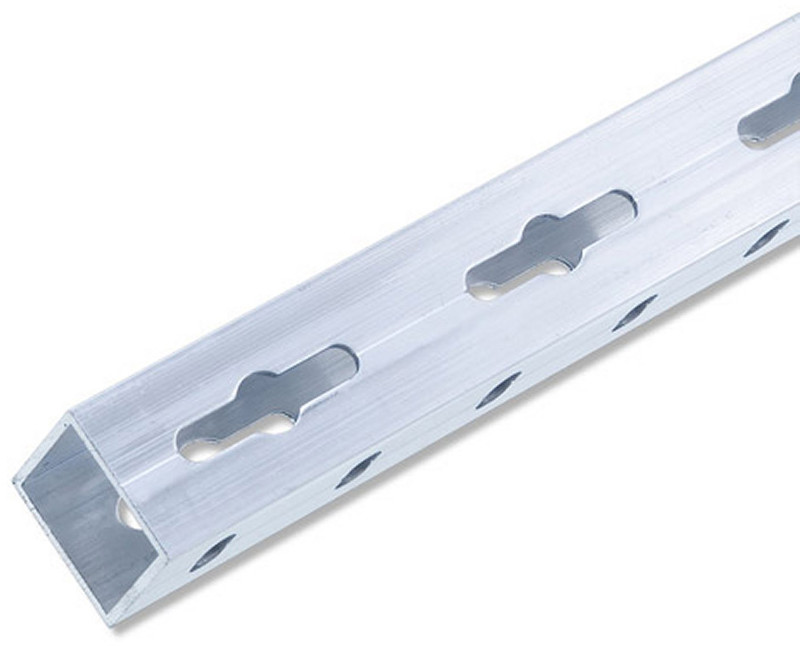
\includegraphics[width=10cm]{img/profile.jpg}}
\end{figure}
La première solution est chère. Il faut compter 60\euro les trois mètres %
(30mm), sans compter la quincaillerie d'assemblage. \par%
La seconde solution, la moins chère, est plus difficile à mettre en %
oeuvre et nécessite de la précision dans les usinages (perçages, sciages, %
...) pour avoir de bons alignements.%
La dernière solution est un bon compromis, car c'est une solution de %
construction modulaire à petit prix (15\euro les 2,5m x 25mm). Les jonctions %
se font avec des L et des T en PVC. Si ce n'est pas assez rigide, je %
pourrais encore ajouter des équerres métaliques.
\subsection{L'électronique}
\subsubsection{Spécification}
L'électronique de commande doit respecter les spécifications suivantes: %
\begin{itemize}%
\item{Elle devra piloter 5 axes (1 X-axis, 1 Y-axis, 2 Z-axis, 1 extrudeur)} %
\item{Elle se connectera à un ordinateur via le port USB} %
\item{Elle supportera une carte SD pour l'imprimante soit autonaume lors de %
l'impression} %
\item{Elle saura piloter des moteurs pas à pas bipolaires}
\item{Elle intégrera les différents capteurs (fin de course, températere de %
l'extrudeur)}
\item{Elle saura piloter le partie chauffante de l'extrudeur} %
\item{Elle ne sera pas propriétaire} %
\end{itemize} %
\subsubsection{La Smoothieboard}
Toujours, pour des questions de budget, j'ai écarté la solution Smoothie %
(http://smoothieware.org/smoothieboard). Il faut compter 125\euro{} pour une %
carte 5 axes.
\subsection{Arduino}
La solution Arduino consiste à utiliser la version Mega et y brancher une carte %
de commande de moteur. Je suis donc parti sur la configuration suivante: %
\begin{itemize}%
\item{Freeduino 2650 Mega (un clone de l'Arduino, mais en moins cher): 19\euro}%
\item{RAMPS (une carte de commande de moteur; la plus utilisée par les firmwares %
proposés): 14\euro}%
\item{5 modules A4988 (commande de moteur pas à pas): 5\euro{} chacun}
\end{itemize}%
%
\subsection{Liste du matériel}
\csvreader[tabular=|l|l|l|r|,
    table head=\hline & Description & Qte & Prix\\\hline,
    late after line=\\\hline]%
{bom.csv}{Description=\Description,Qte=\Qte,Prix=\Prix}%
{\thecsvrow & \Description & \Qte & \Prix}%